% TEX program = xelatex
%%
%% This is file `sample-sigconf.tex',
%% generated with the docstrip utility.
%%
%% The original source files were:
%%
%% samples.dtx  (with options: `sigconf')
%% 
%% IMPORTANT NOTICE:
%% 
%% For the copyright see the source file.
%% 
%% Any modified versions of this file must be renamed
%% with new filenames distinct from sample-sigconf.tex.
%% 
%% For distribution of the original source see the terms
%% for copying and modification in the file samples.dtx.
%% 
%% This generated file may be distributed as long as the
%% original source files, as listed above, are part of the
%% same distribution. (The sources need not necessarily be
%% in the same archive or directory.)
%%
%% The first command in your LaTeX source must be the \documentclass command.

\documentclass[sigconf]{acmart}
\newcommand{\B}{\fontseries{b}\selectfont}
\usepackage[ruled,linesnumbered]{algorithm2e}
\usepackage{svg}
\usepackage{amsmath}
\usepackage{epstopdf}
%% NOTE that a single column version is required for 
%% submission and peer review. This can be done by changing
%% the \doucmentclass[...]{acmart} in this template to 
%% \documentclass[manuscript,screen]{acmart}
%% 
%% To ensure 100% compatibility, please check the white list of
%% approved LaTeX packages to be used with the Master Article Template at
%% https://www.acm.org/publications/taps/whitelist-of-latex-packages 
%% before creating your document. The white list page provides 
%% information on how to submit additional LaTeX packages for 
%% review and adoption.
%% Fonts used in the template cannot be substituted; margin 
%% adjustments are not allowed.

%%
%% \BibTeX command to typeset BibTeX logo in the docs
\AtBeginDocument{%
  \providecommand\BibTeX{{%
    \normalfont B\kern-0.5em{\scshape i\kern-0.25em b}\kern-0.8em\TeX}}}

%% Rights management information.  This information is sent to you
%% when you complete the rights form.  These commands have SAMPLE
%% values in them; it is your responsibility as an author to replace
%% the commands and values with those provided to you when you
%% complete the rights form.
\setcopyright{acmcopyright}
\copyrightyear{2021}
\acmYear{2021}
%\acmDOI{10.1145/1122445.1122456}

%% These commands are for a PROCEEDINGS abstract or paper.
\acmConference[KDD'21]{}{14-18 August}{ Singapore}
%\acmBooktitle{Woodstock '18: ACM Symposium on Neural Gaze Detection,
 % June 03--05, 2018, Woodstock, NY}
%\acmPrice{15.00}
%\acmISBN{978-1-4503-XXXX-X/18/06}


%%
%% Submission ID.
%% Use this when submitting an article to a sponsored event. You'll
%% receive a unique submission ID from the organizers
%% of the event, and this ID should be used as the parameter to this command.
%%\acmSubmissionID{123-A56-BU3}

%%
%% The majority of ACM publications use numbered citations and
%% references.  The command \citestyle{authoryear} switches to the
%% "author year" style.
%%
%% If you are preparing content for an event
%% sponsored by ACM SIGGRAPH, you must use the "author year" style of
%% citations and references.
%% Uncommenting
%% the next command will enable that style.
%%\citestyle{acmauthoryear}

%%
%% end of the preamble, start of the body of the document source.
\begin{document}

%%
%% The "title" command has an optional parameter,
%% allowing the author to define a "short title" to be used in page headers.
\title{Fea2Fea : Feature to Feature Prediction and Augmentation on Small Graphs}

%%
%% The "author" command and its associated commands are used to define
%% the authors and their affiliations.
%% Of note is the shared affiliation of the first two authors, and the
%% "authornote" and "authornotemark" commands
%% used to denote shared contribution to the research.

\author{Jiaqing Xie}
\affiliation{%
  \institution{University of Edinburgh}
  %\streetaddress{1 Th{\o}rv{\"a}ld Circle}
  \city{Edinburgh}
  \country{United Kingdom}}
%\email{s2001696@ed.ac.uk}

\author{Rex Ying}
\affiliation{%
  \institution{Stanford University}
  %\city{Rocquencourt}
  \country{USA}
}


%%
%% By default, the full list of authors will be used in the page
%% headers. Often, this list is too long, and will overlap
%% other information printed in the page headers. This command allows
%% the author to define a more concise list
%% of authors' names for this purpose.
%\renewcommand{\shortauthors}{Trovato and Tobin, et al.}

%%
%% The abstract is a short summary of the work to be presented in the
%% article.
\begin{abstract}
 
\end{abstract}

%%
%% The code below is generated by the tool at http://dl.acm.org/ccs.cfm.
%% Please copy and paste the code instead of the example below.
%%

%%
%% Keywords. The author(s) should pick words that accurately describe
%% the work being presented. Separate the keywords with commas.
\keywords{datasets, neural networks, gaze detection, text tagging}

%% A "teaser" image appears between the author and affiliation
%% information and the body of the document, and typically spans the
%% page.


%%
%% This command processes the author and affiliation and title
%% information and builds the first part of the formatted document.
\maketitle

\section{Introduction}

\begin{figure}[!h]
    \centering
    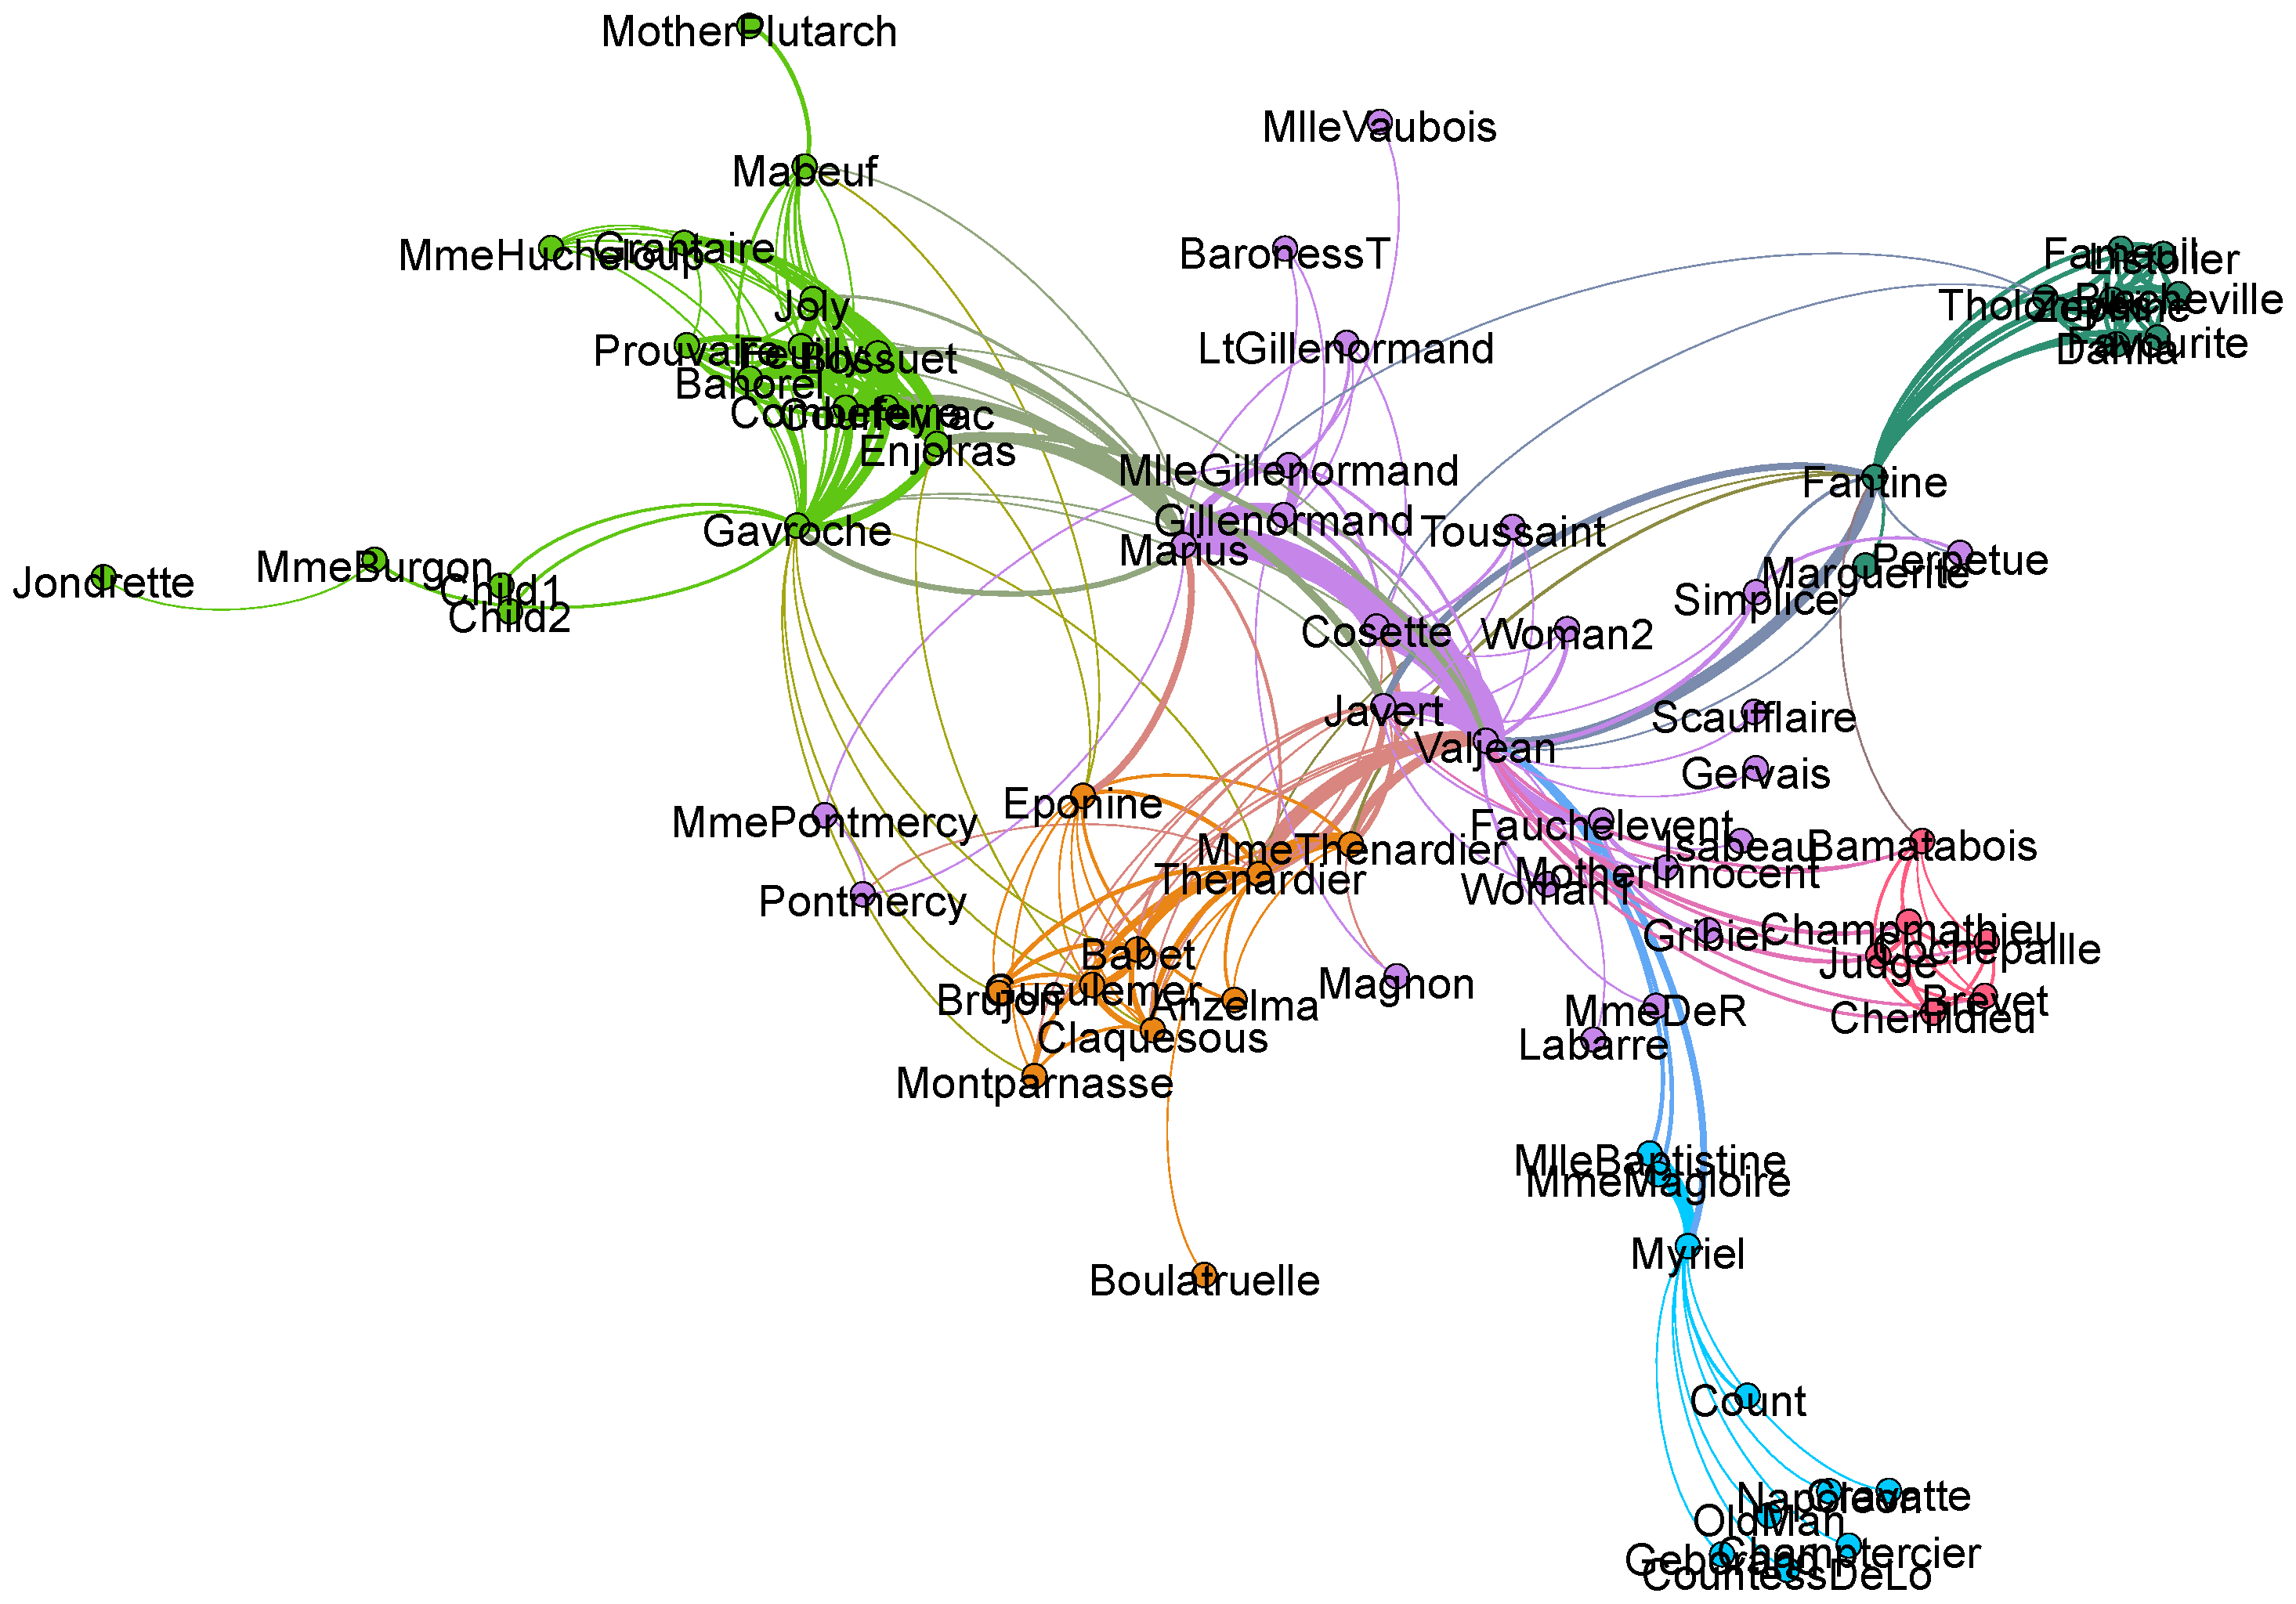
\includegraphics[width = 0.45\textwidth]{fig/LesMiserables.eps}
    \caption{Question: In LesMiserables dataset, if already know the character Valjean has 35 neighbours(degrees), can we predict the feature PageRank of Valjean through graph neural network?) }
\end{figure}

\begin{figure*}
    \centering
    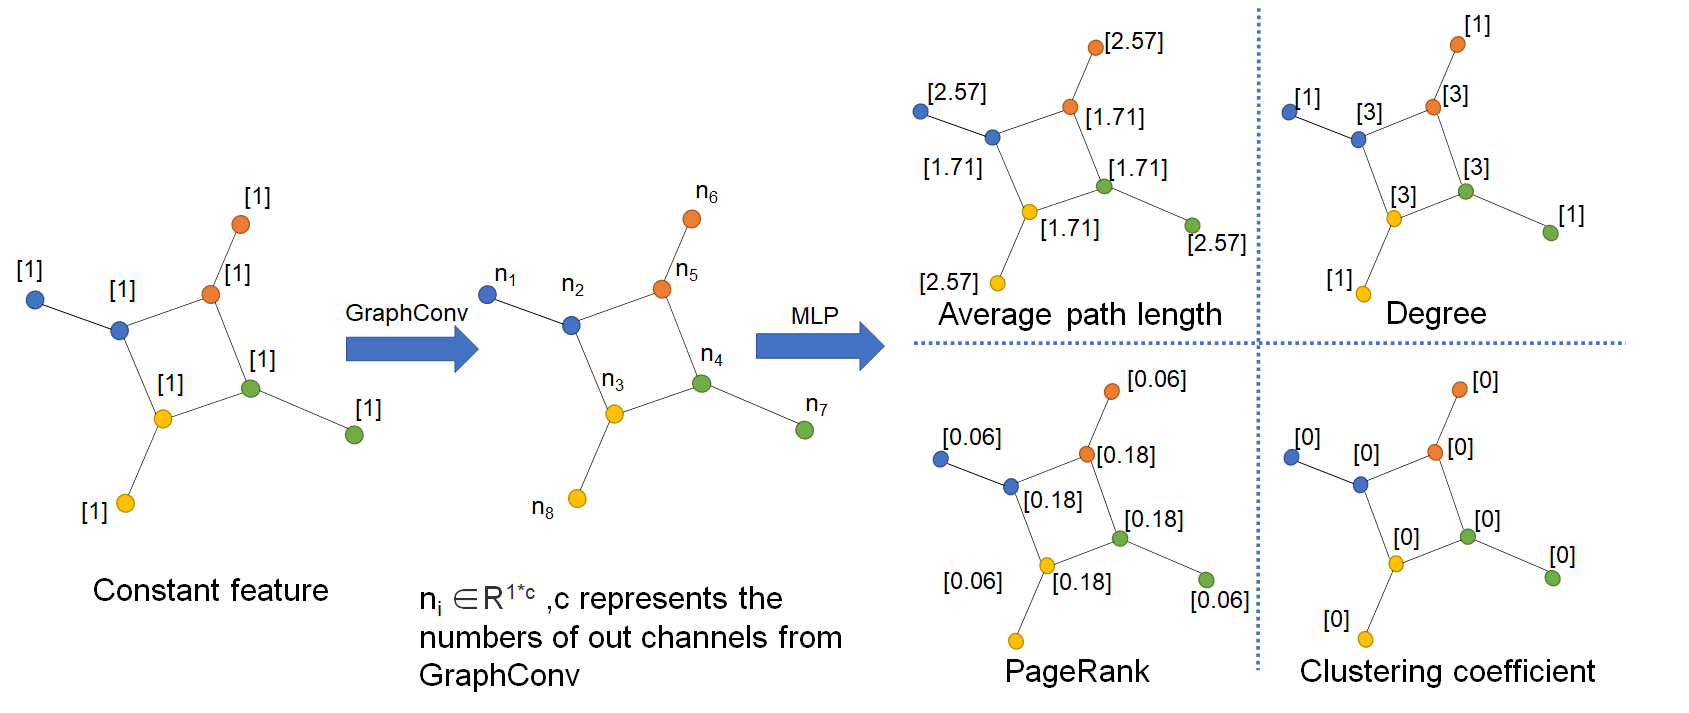
\includegraphics[width=1\textwidth]{Pipeline.jpg}
    \caption{Baeline model for feature mutual prediction task}
\end{figure*}


 Graph neural networks(GNN) are widely used in node classification, graph classification, link prediction problems and graph embedding extractions. Graph neural networks have broad application scenarios including knowledge graph, social network, computer network and also recommender systems. Better learning of graph structures and comprehensive learning of features' relationship on those tasks and application scenarios based on GNN might enable researchers to make predictions precisely. In a regular graph classification task, adjacency matrix and feature matrix are considered as the default inputs of a graph neural network. For example, benchmark Cora dataset has an input feature matrix F  $\in \mathbb{R}^{2708 \times1433}$ where it represents 2708 papers with 1433 filtered words for each paper entry, and it also has an adjacency matrix A$ \in \mathbb{R}^{2708 \times2708}$, 
where each element represents the link information between each two papers (both 0-1 matrix). Graph properties are not added to our input but instead sometimes we analyze them alone by taking each property into consideration. By giving an directed or undirected graph, we can easily get the property of degree of each node or the nodes' clustering coefficients by counting edges but we do not predict them at all, which means the prediction objects are always the nodes' or graph's classes. We do not know if adding those properties can help improve node or graph classification accuracy or not, or if there exists a strong relationship between features or not. 

In this paper, we build models that are based on various kinds of graph convolutional layer types, including Graph Attention Netowrk(GAT), GraphSAGE, Graph Isomorphic Network(GIN) and Graph Convolutional Network(GCN) with multi-layer perceptron to perform mutual feature predictions instead of node classifications on the benchmark dataset to see the relationship between features. The features that selected for our research are  constant feature, node degrees, clustering coefficient, average path length and pagerank. We choose Planetoid, TUDataset, Reddit and PPI dataset for the research and also include the random generated graph for further validation. If one feature predict the other feature precisely, they are considered to be redundant to concatenated features' representation.  Finally we insert our artificial generated features to see which combination is the best, which is the feature augmentation period. Different datasets may have different feature combinations to augment their feature representations.   



We design totally different experiments instead of traditional graph classification or link prediction problems in order to know features' relationship: (i) feature to feature prediction (ii) concatenated features to feature prediction (iii) original features with concatenated features to feature prediction(augmentation). Our task is to know (i) if GNN can perform these tasks well, including our own models, to test if GNN is powerful at predicting everything related (ii) of which features are closely related according our predictions, high value means redundant (iii) do augmentation really works on mutual feature prediction (iv) to see if node tasks and graph tasks are both effective to augmentation.

\section{Related Works}



\subsection{Graph Representation Learning}

\subsection{Feature Importance}

\section{Methods}


\subsection{Baseline Graph embedding methods}
\paragraph{GCN} GCN is the abbreviation of \textbf{Graph Convolutional Network}\cite{kipf2016semi}. It derives from  signal processing domain which takes the advantage of Laplacian matrix representation and filters by applying fourier transforms to graph signals. Here's the propagation rule of a multi-layer GCN: 
\begin{equation}
\setlength\abovedisplayskip{5pt}%shrink space
\setlength\belowdisplayskip{5pt}
X^{\left(l+1\right)} = \sigma\left(\widetilde D^{-\frac{1}{2}} \widetilde A \widetilde D^{-\frac{1}{2}} X^{(l)} W^{(l)}\right)\\
\end{equation}
$X^{(l)} \in  \mathbb R^{N_{l} * D_{l}}$ is the input of layer $(l+1)$, where $X^{(0)}$ is the initial feature matrix of the graph. $\widetilde D_{ii} = \sum_{j}\widetilde A_{ij}$ is a learnable degree matrix and $W^{(l)}$ is a learnable weight matrix. $\widetilde A = I_{n} + A$ is an adjacency matrix with self-connection and $I_{n}$ is the identity matrix. It performs normalization to alleviate gradient vanishing problems.  GCN has the time complexity of $O(V)$ where V is equal to number of nodes if adjacency matrix $\widetilde 
A$ is sparse. GCN embedding is more efficient in small graphs than large graphs. It's a transductive method which takes the whole graph into account. However, it's not influential when encoding small graphs that we want to explore.

\paragraph{GraphSAGE}  GraphSAGE is an inductive graph representation learning method\cite{hamilton2017inductive}, which performs better than transductive methods such as GCN on large graphs. According to small graphs, they might show no difference on running time. The iteration of graph representation is computed by the aggregation of neighbourhood message of a given node, not considering all the edges in the graph. It concatenates itself to the message passing from its neighbours at k-th iteration with an MLP:
\begin{equation}
\setlength\abovedisplayskip{5pt}%shrink space
\setlength\belowdisplayskip{5pt}
h_{v}^{(k)} = \sigma\left(\mathbf{W}^{(k)} \cdot \textup{\small CONCAT} \left(h_{v}^{(k-1)},h_{\mathcal N\left(v\right)}^{(k)}\right)\right), v \in \mathcal V\\ 
\end{equation}
Here $h_{v}^{(k)}$ is the representation of node v at k-th iteration. $h_{\mathcal N\left(v\right)}^{(k)}$ is the aggregation of node v's neighbours at k-th iterarion. $\mathbf{W}^{(k)}$ is the trainbale weight matrix at k-th iteration. $\sigma\left( \cdot \right)$ is the activation function. The nearby nodes show similar output structures while disparate nodes have totally different representations\cite{hamilton2017inductive}. Aggregation methods include mean, maxpooling, sum and LSTM aggregator\cite{hamilton2017inductive}.

\paragraph{GIN}  GIN is the abbreviation of \textbf{Graph Isomorphism Network}\cite{xu2018powerful}. Experiments show that GIN is as powerful as WL test, which can differentiate two different graph structures and identify two isomorphic graphs. Consider the propagation rule of GIN:
\begin{equation}
\setlength\abovedisplayskip{5pt}%shrink space
\setlength\belowdisplayskip{5pt}
h_{v}^{(k)} = \textup{MLP}^{(k)}\left( \left( 1 + \varepsilon^{(k)}\right) \cdot h_{v}^{(k-1)} + \sum\nolimits_{u \in \mathcal N(v)} h_{u}^{(k-1)}\right)  \\
\end{equation}
Here $h_{v}^{k}$ is the representation of node v at k-th iteration. It can be also written by $f\circ\varphi$. {\sc Gin} uses MLP to learn $f$ and $\varphi$. Injective function avoids two multisets generate the same embeddings from GNN. Meanwhile, similar graph embeddings have similar embeddings in GIN. Output module is essential in GIN, which includes a concatenation process and a readout module. Readout module is sum in GIN, while max and mean dissatisfy injective property. GraphSAGE embedding with mean aggregator performs as well as GIN. They have great performance on graph but not generally on node classification.





\paragraph{GAT} GAT is the abbreviation of \textbf{Graph Attention Network}\cite{velivckovic2017graph}. It takes the advantage of attention mechanism, which is first proposed in a transformer architecture in NLP domain. The attention weight between node i and one of its neigbours node j can be expressed as $\alpha_{ij}$: 
\begin{equation}
\setlength\abovedisplayskip{5pt}%shrink space
\setlength\belowdisplayskip{5pt}
\alpha_{ij} = \frac{\textup{exp}\left(\textup{LeakyReLU}\left(\vec{\mathbf{a}}^{T}[\mathbf{W}\vec{h_{i}}||\mathbf{W}\vec{h_{j}}]\right)\right)}{\sum_{k \in \mathcal N\left(i\right)}\textup{exp}\left(\textup{LeakyReLU}\left(\vec{\mathbf{a}}^{T}[\mathbf{W}\vec{ h_{i}}||\mathbf{W} \vec{h_{k}}]\right)\right)}\\
\end{equation}
Here it performs softmax operation. $\vec{h_{i}^{'}}$ is the node embedding of node i.$\vec{h_{j}^{'}} \in \mathbb{R}^{F'}$
is representation of one of node i's neighbours. $\vec{\mathbf{a}}^{T} \in \mathbb{R}^{2F'}$ is parameterized weight vector. LeakyReLU is a non-linear activation function. Output feature is $\vec{h_{i}'}$:
\begin{equation}
\setlength\abovedisplayskip{5pt}%shrink space
\setlength\belowdisplayskip{5pt}
\vec{h_{i}'} = \sigma\left(\sum_{j \in \mathcal N_{i}}\alpha_{ij}\mathbf{W}\vec{h_{j}}\right)\\
\end{equation}
It'a a linear combination with non-linearity $\sigma(\cdot)$. The combination method of multi-head attention in GAT is take averaging result. The advantage of GAT is that we can perform inductive learning without knowing everything about the whole graph.

\subsection{Feature to Feature Approach}

\begin{algorithm}
\caption{Get Matrix of Feature Mutual Relationship}
\KwIn{Graph $\mathcal G$($\mathcal V, \mathcal E$);  node property length $\mathcal K$; Input property matrix   $\mathbf{x}_{\mathcal{G}}\in\mathbb{R}^{|\mathcal{V}|\times \mathcal{K}} $, second dimension order is constant feature, degree, clustering coefficient, pagerank and average path length; model architecture $\mathcal M$, including GNN embedding(GCN, GraphSAGE, GIN, GAT) with MLP model; metrics $\mathcal P$ }
\KwOut{ Feature mutual relationship matrix $\mathcal R \in \mathbb{R}^{\mathcal K \times \mathcal K}$}
$\mathcal R \gets 0$\\
\For{$i \gets 1$ \textbf{to} $\mathcal K$}{
    $\mathcal R(i,i) \gets 1$\\
    $\textbf{I}_{\mathcal G} \gets \textbf{x}_{\mathcal G}(:,i)$\\
    \If{i == $\mathcal{K}$}{
    \Return{$\mathcal R$}\;
    }
    \For{ $j \gets i + 1$ \textbf{to} $\mathcal K$
    }{

    $\textbf{O}_{\mathcal G} \gets \textup{Bin}\left(\textbf{x}_{\mathcal G}(:,j)\right)$\\
    $\textbf{O}^{'}_{\mathcal G} \gets$ $\mathcal{M}\left(\textbf{I}_{\mathcal G}, \textbf{O}_{\mathcal G}\right)$\\
    $\mathcal{R}(i,j), \mathcal{R}(j,i) \gets \mathcal P(\textbf{O}^{'}_{\mathcal G},\textbf{O}_{\mathcal G} )$
    }
}
\end{algorithm}

The task for the graph feature to feature prediction is implemented by baseline models, aiming to test a GNN model's robustness on small graphs. Here the input is one signal feature $\mathbf{x}_{\mathcal{G}}$




\subsection{Feature Concatenation Methods}

\paragraph{SkipLast}


\paragraph{Concatenation by importance}

\paragraph{Inner Product Concatenation}




\subsection{}


\section{Experimemts}

\begin{figure*}[!htbp]
\centering
\begin{center}
 \hspace*{-1.5in}
    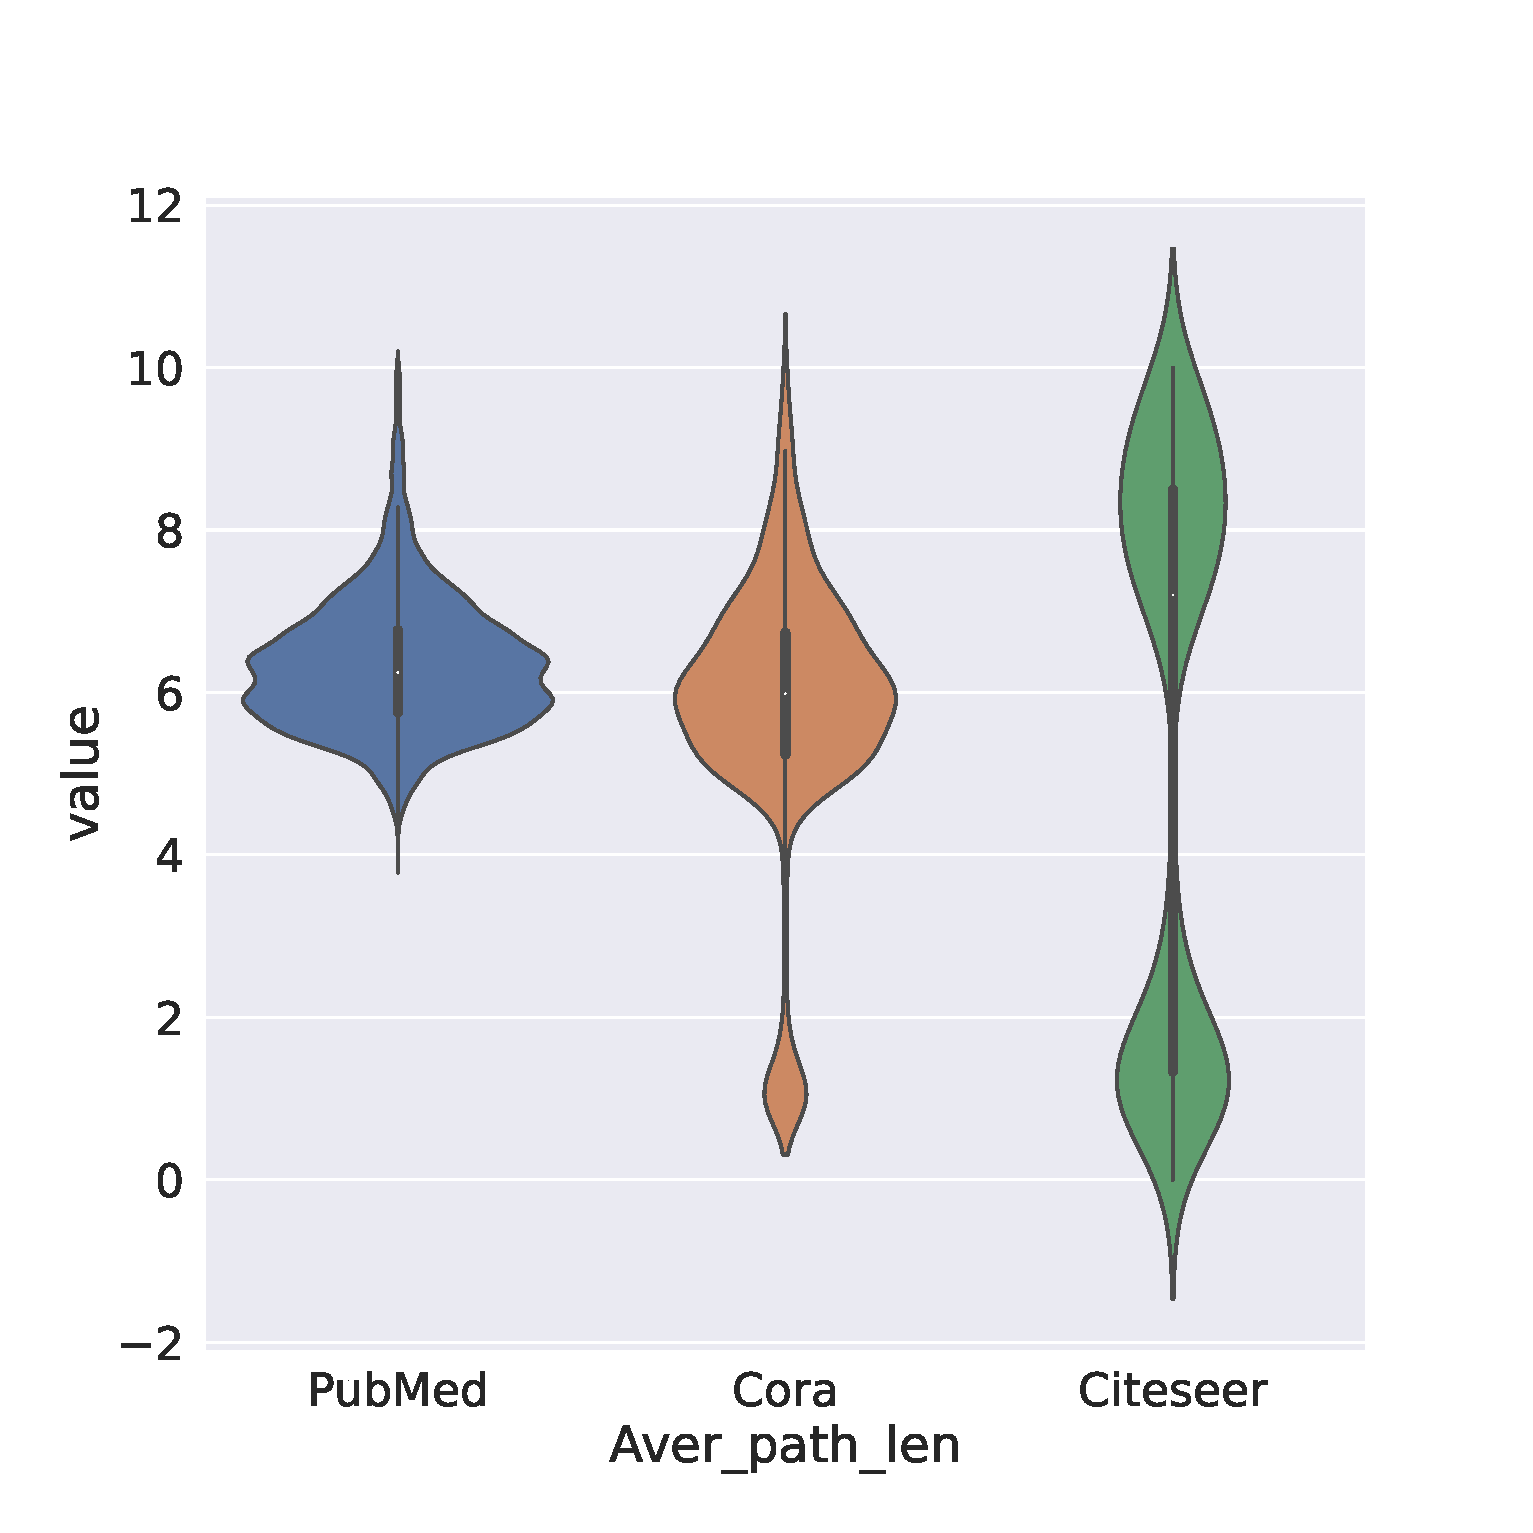
\includegraphics[width=0.27\linewidth]{fig/Aver_path_len_planetoid_vp.eps}
    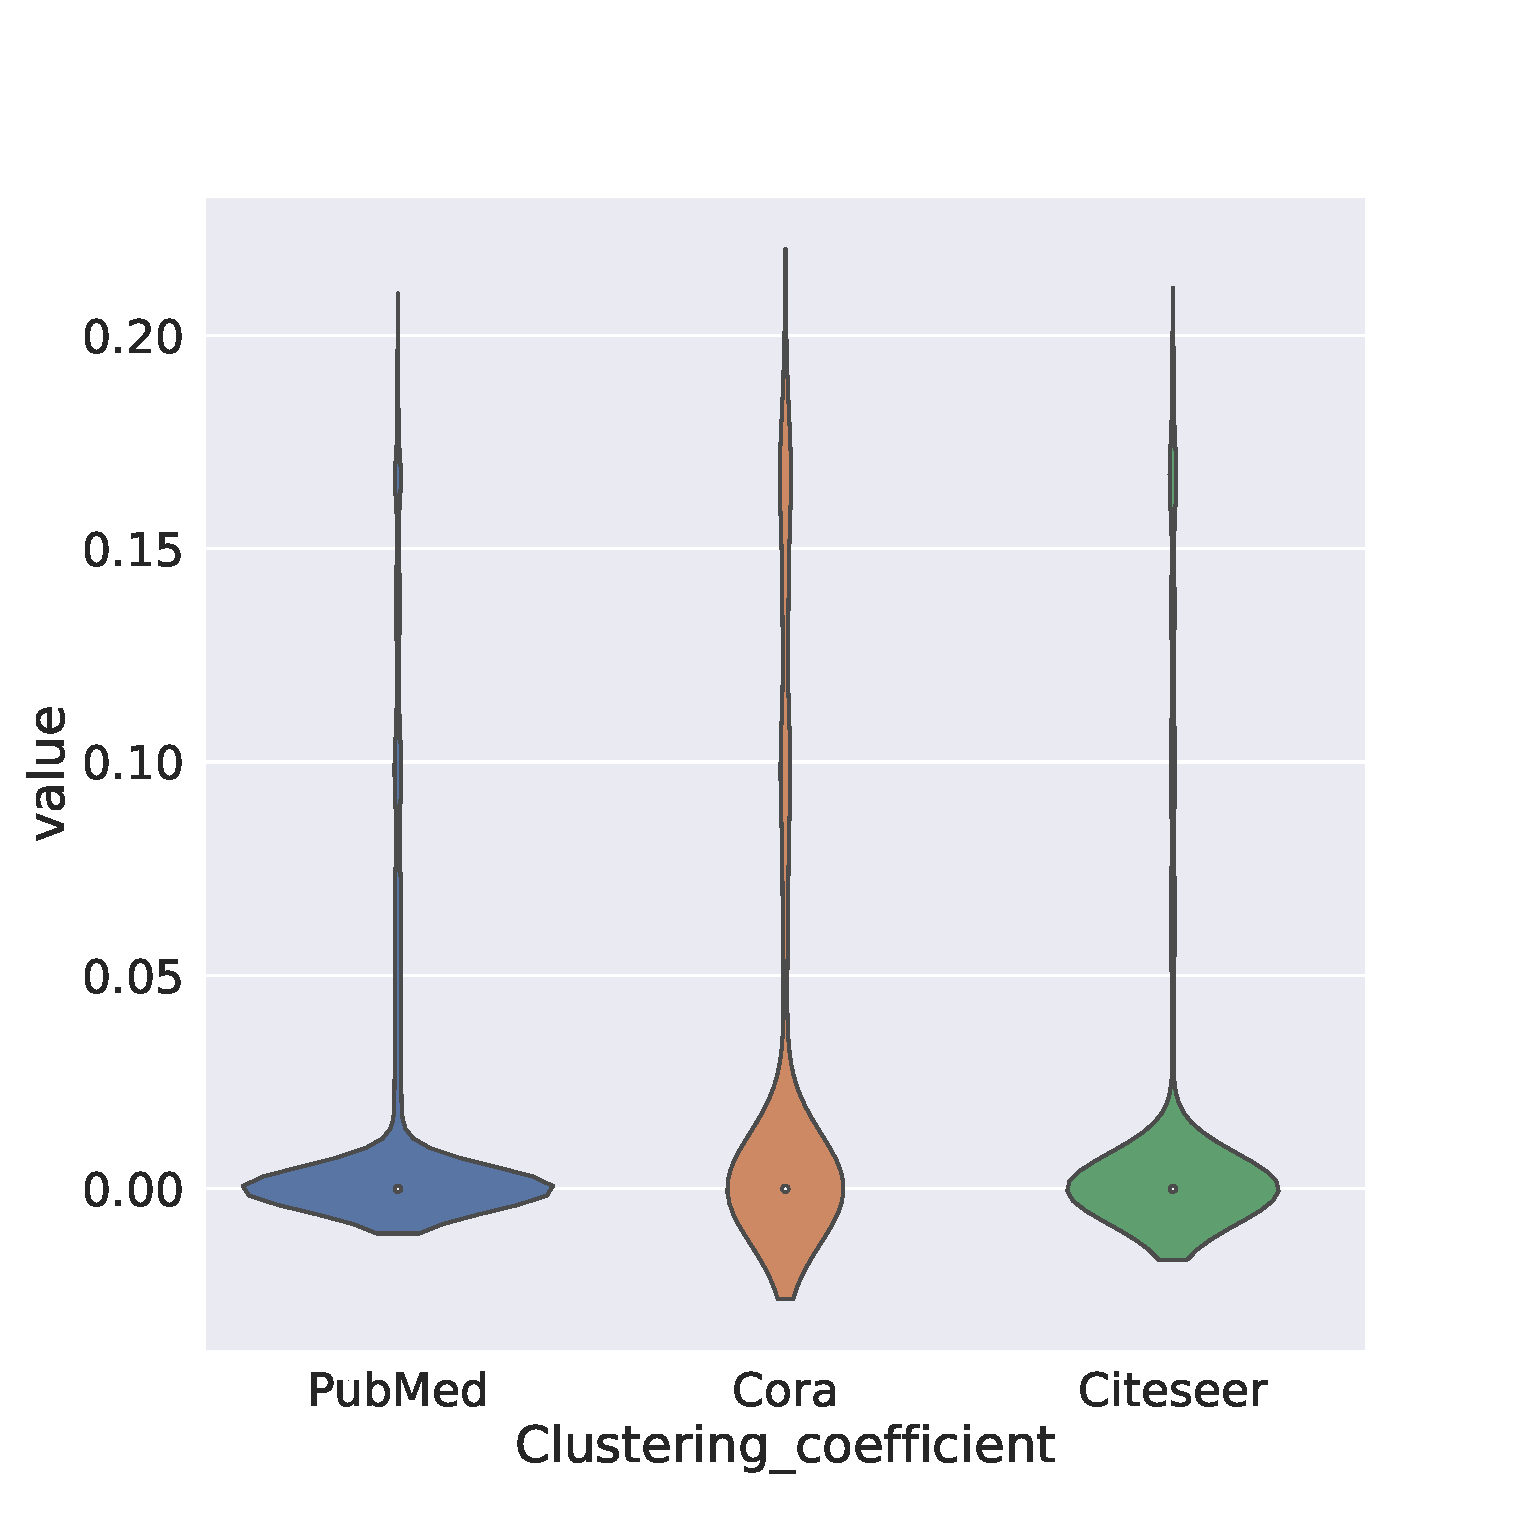
\includegraphics[width=0.27\linewidth]{fig/Clustering_coefficient_planetoid_vp.eps}
    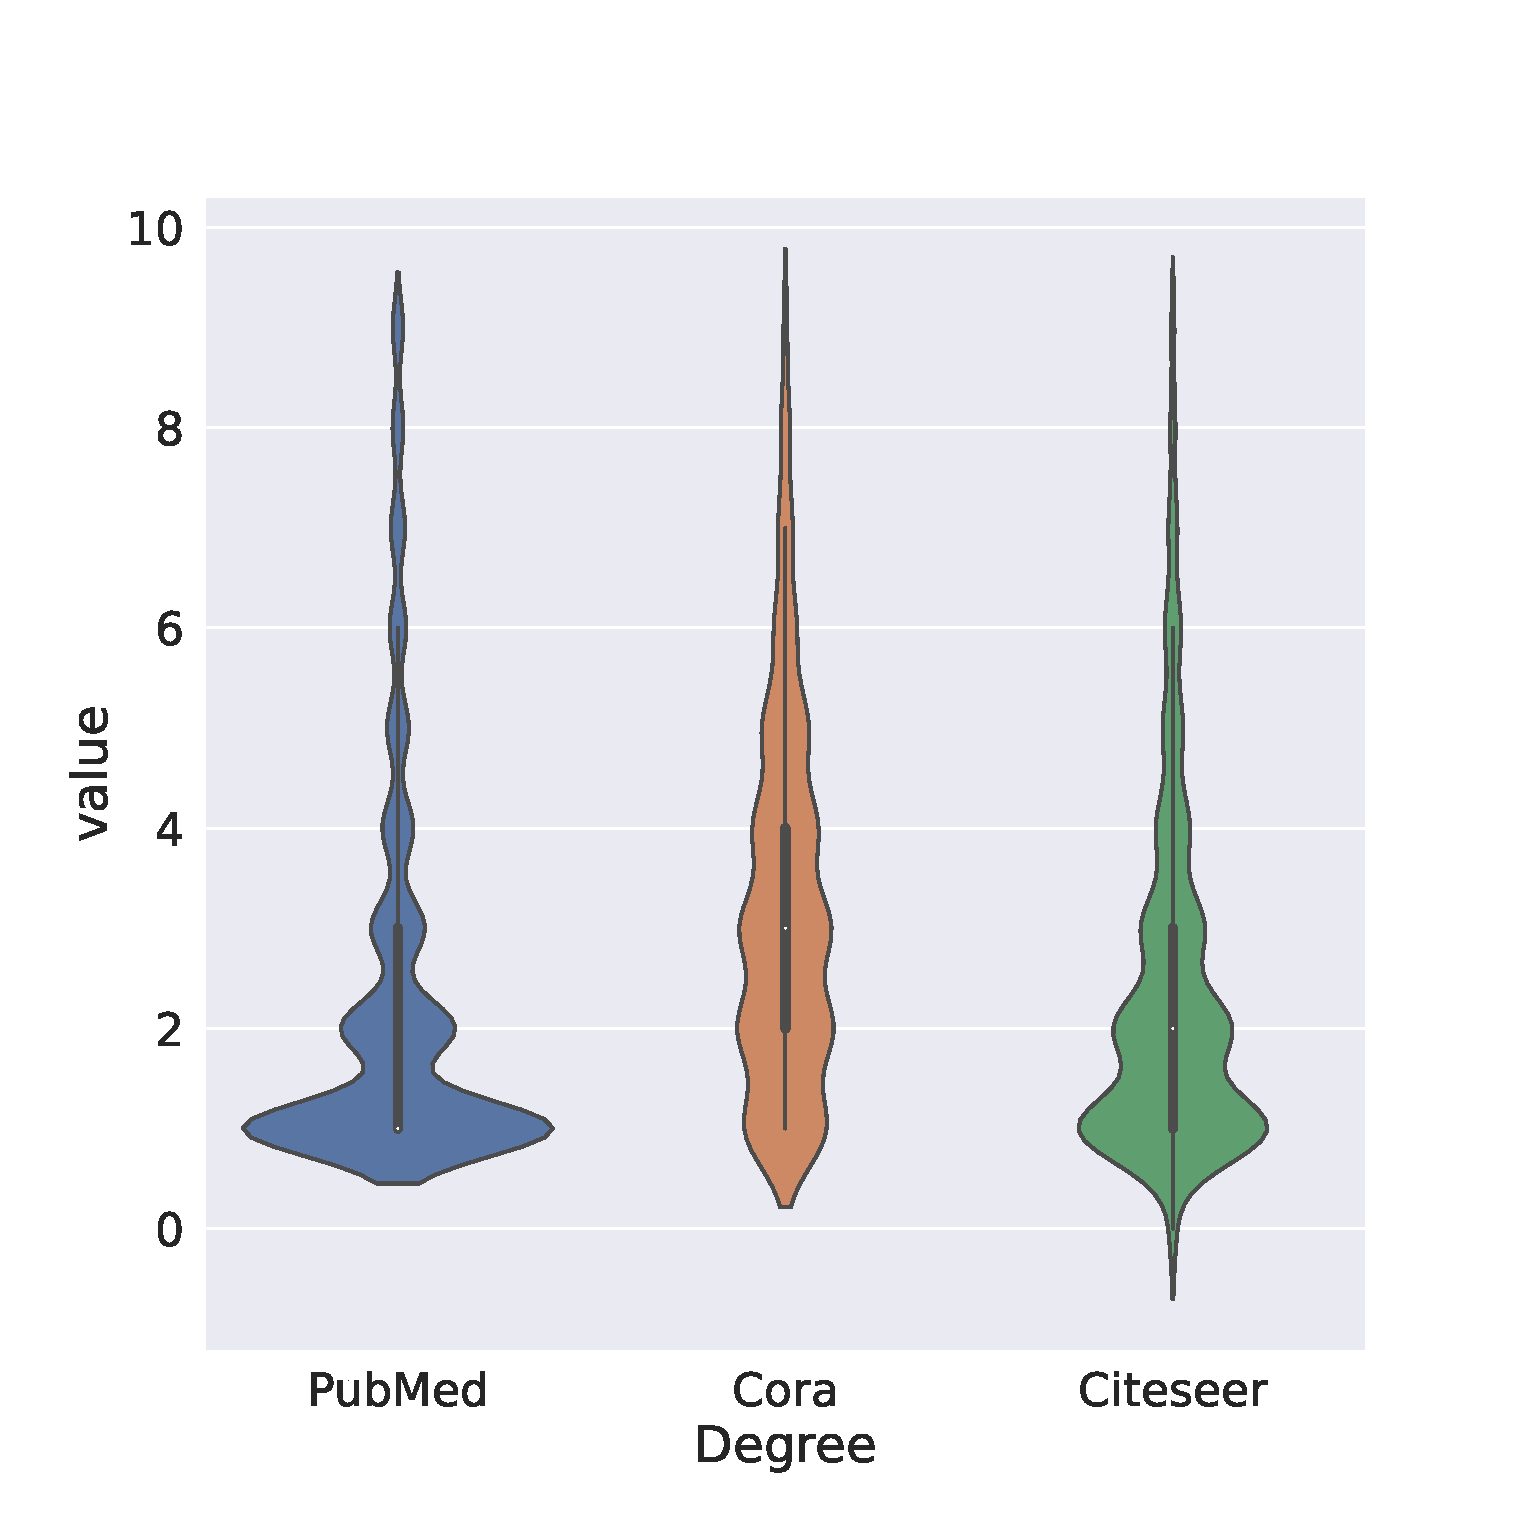
\includegraphics[width=0.27\linewidth]{fig/Degree_planetoid_vp.eps}
    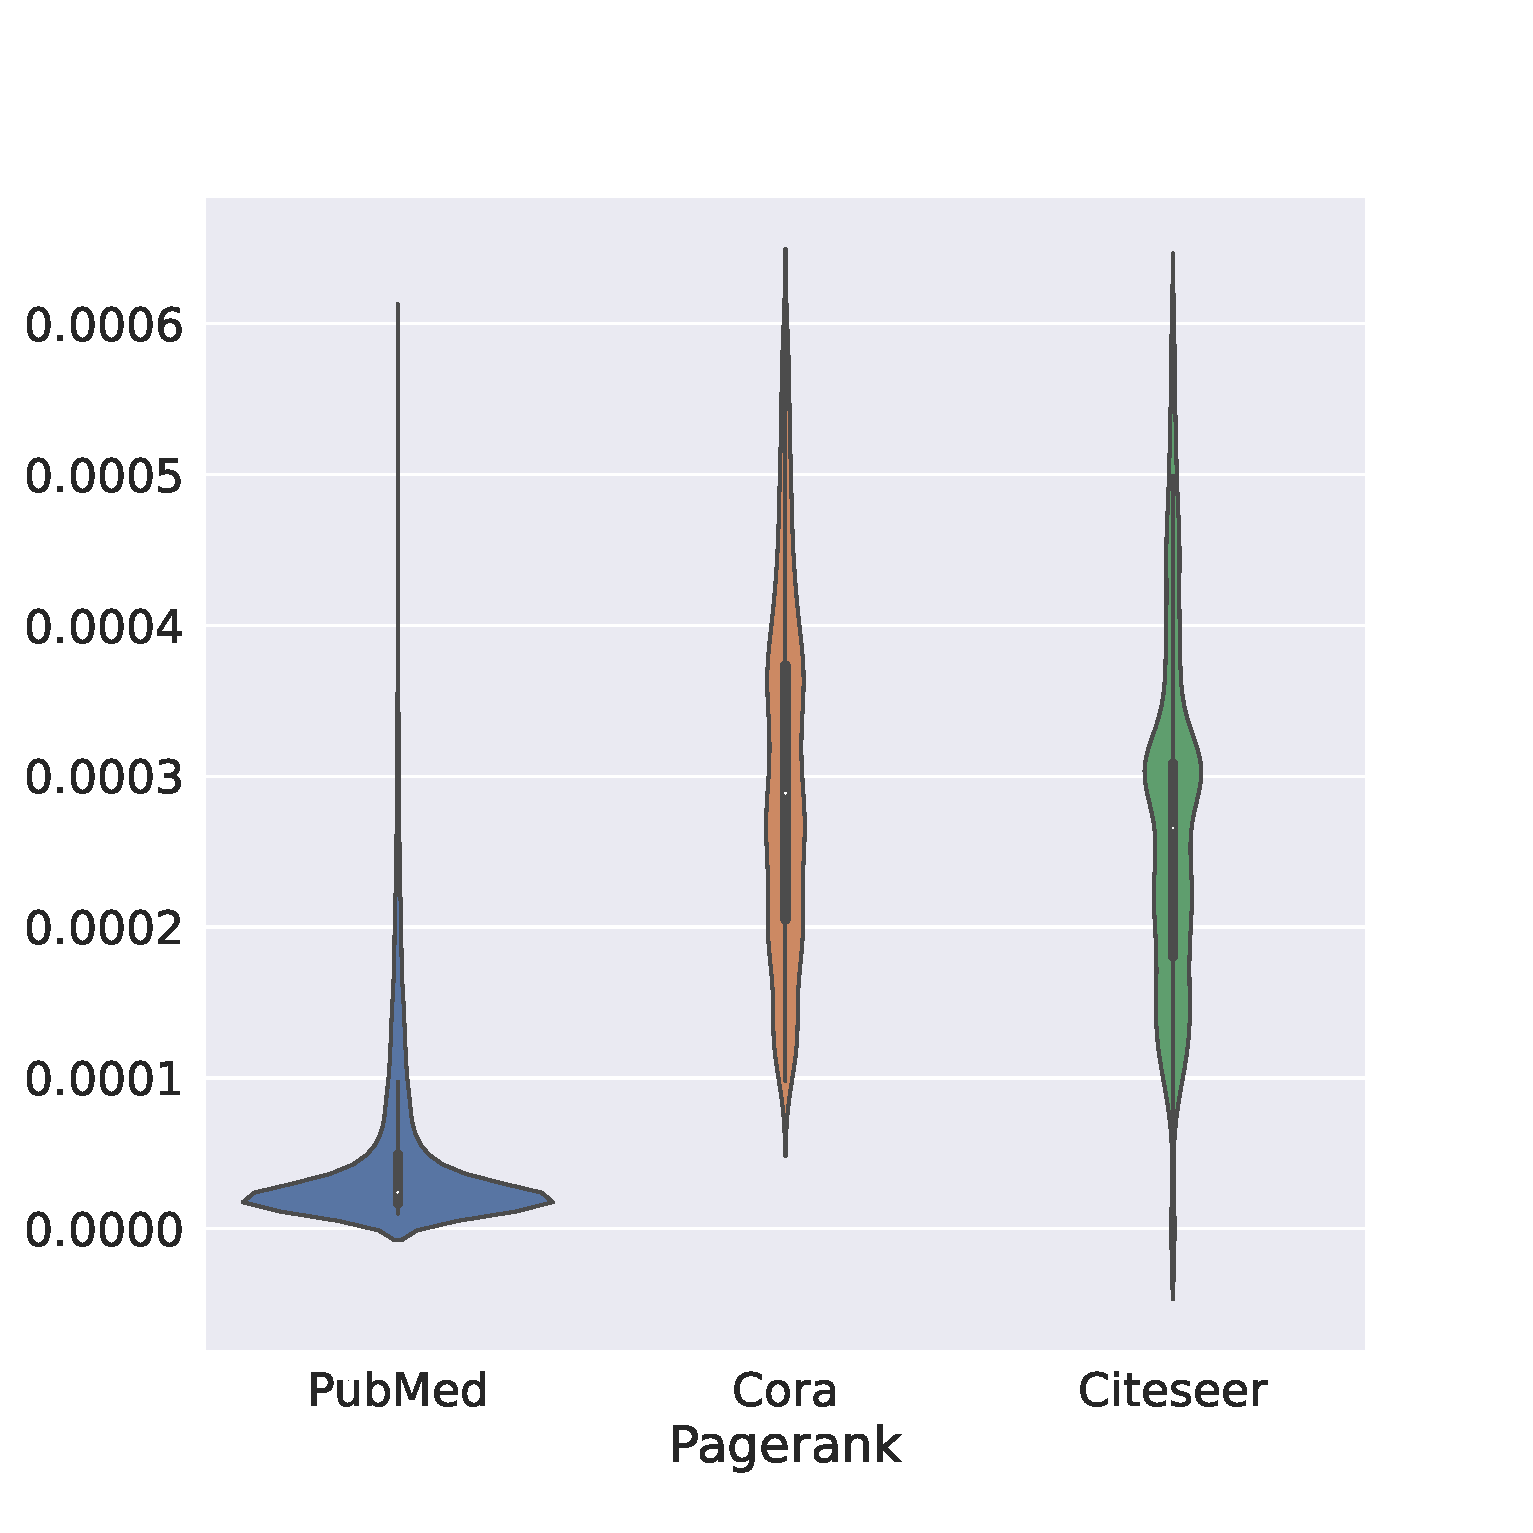
\includegraphics[width=0.27\linewidth]{fig/Pagerank_planetoid_vp.eps}
    \hspace*{-1.5in}
    \caption{Violin plots of graph properties on planetoid datasets}
\end{center}
\end{figure*}



We compute the feature matrices for each graph. We implement four graph embedding methods: GIN, GCN, GraphSAGE and GAT on graph feature inputs to predict features' relationship matrices, which is regarded as the traditional GNN result on new tasks. We also compare them with the added GNN blocks that we have designed, as the comparison of GNN models in order to interpret Graph Neural Network's robustness. We've also handled with some important issues in the following parts. Typical datasets that meet the requirement of small graphs are listed in 4.1. Coding environment settings and parameter settings are detailed in 4.2. 

\subsection{Datasets}
In our preliminary experiments, we choose ten small graph-based datasets. A generation of supervised graph is also included. However, according to the data that mentioned in original GraphSage
paper, which are the aimed large graph, we do not care about them at this stage.
\paragraph{Planetoid}
Planetoid datasets are citation datasets including {\sc Cora}, {\sc CiteSeer} and {\sc PubMed}. One node in the graph represents each paper. Edge index means there is a citation link between two papaers and nodes in the graph are undirectly linked. The feature matrix of each dataset is given by sparse bags-of-words vectors. It's one-hot encoding which is at a lower level embedding space. In  {\sc Cora} dataset, there are 2708 nodes with 1433 features and 5429 edges. In {\sc CiteSeer} dataset, there are 3327 nodes with 3703 features and 4732 edges. In {\sc PubMed} dataset, there are 19717 nodes with 500 features and 44338 edges. In this work, we choose all of three datasets to show the generalization effects, which is that firstly we test on {\sc Cora} dataset, then we test on {\sc CiteSeer} and {\sc PubMed}.

\paragraph{TUDataset}
TUDataset is a collection of benchmark datasets for learning graph representations, which gathers numerous domains and is authored by different experts. More specifically, it includes data from small molecules, bioinformatics, social networks, computer vision and other synthetic kernels. In this work, we choose two datasets  {\sc Proteins} and {\sc Enzymes} from Bioinformatics domain. In {\sc Enzymes} dataset, there are 600 graphs with 6 classes. Each graph has an average edges of 62.1 and an average edges of 32.6. In {\sc Proteins} dataset, there are 1113 graphs with 2 classes. Each graph has an average egdes of 39.1 and an average edges of 72.8. We will make more experiments on other datasets, such as {\sc Zinc} and {\sc Qm9} from molecular datasets or {\sc Reddit-Binary} and {\sc Reddit\_Threads} from social networks. 

\paragraph{PPI}
Protein to Protein Interaction(PPI) network is generally used in biochemistry, containing positional gene sets, motif gene sets and immunological signatures as features (50 in total) and gene ontology sets as labels (121 in total). It is mentioned in this paper. 

\subsection{Experiment Set-up}
We've mentioned four graph embedding methods, which are GCN, GraphSAGE, GIN and GAT. 
Our baseline model is constructed by using graph embeddings and followed by MLPs. We take 

In single feature to feature prediction tasks, we set up a 2-layer GNN with each layer followed by \textit{batch norm}
layer, activated by\textit{relu function} and using \textit{dropout} method. Especially  





Add parameter setting and coding environment here:\\

We mainly use Pytorch framework together with torch\_geometric API for building our model architecture.  In the single feature to single feature task, our default model consists of two GNN blocks and a MLP block with two linear layers. We both have classification tasks for feature prediction and also regression tasks. The metrics for classification task is the accuracy score and macro-F1 score. Input dimension is set to 1 which is input\_channel parameter. 

\subsection{Feature properties of graphs}
We choose five of all graph features to show exploratory results, which are constant feature(Cons), degree(Deg), clustering coefficient(Clu), average path length(AvgLen) and PageRank(PR).

Given a graph $\mathcal{G}$($\mathcal{V}$, $\mathcal{E}$), constant feature of one node u $\mathop{Cons}\limits_{u \in \mathcal{V}}(u)$ is given by c, where c is equal to a constant value. We set to 1 in this project for normalization. Degree of node u $\mathop{Deg}\limits_{u \in \mathcal{V}}(u)$ is equal to the number of node u's neighbours. Clustering coefficient of node u $\mathop{Clu}\limits_{u \in \mathcal{V}}(u)$ = $\frac{2e_{jk}}{k_{i} * (k_{i} - 1)}$, where $j,k \in \mathcal{V}$,$e_{jk}$ represents the total possible edges between node u's neighbours and $k_{i}$ is the number of node u's neighbours.

Having the prerequisite of these basic knowledge, we compute the feature matrix for each dataset. The feature matrix serves to $\mathcal{R}^{|V|*5}$. We should bear in mind that this feature matrix is both used for input and output, as described in Algorithm 1. One important step before fed into training session is to measure the distribution of each feature. Just as imbalanced data is not favoured in the graph or node classification tasks, we observe all the feature distributions and illustrate potential issues among all datasets.


\paragraph{binning methods} Suppose the clustering coefficient is the feature that we want to predict. Clustering coefficient is a non-integer value as we've discussed before. We firstly take it as the classification problem. Binning methods is then used to identify the     Therefore we set bins in order to change the outputs to integers. Figure 2 shows the graph properties on planetoid datasets with violin plots. The property order is: degree, clustering coefficient, pagerank and average path length. Density distribution is very different between each dataset and each property as well. Generally, we set 4-8 bins. Too large bins may lead to a more sparse confusion matrix while too small bins may lead to over concentration on one class. So the number of bins should be not too big nor too small and the number of 4 to 8 satisfies this condition. Specifically, we take the Cora dataset as an example to illustrate the point. Figure 3 shows the example of the property's density distribution on Cora dataset with distplots. We can set 4 bins for Degree, Clustering\_coefficient, Pagerank and Aver\_path\_len according to the values that shown on the x axis of the distplots. 

Through the violin plot we find that most of the clustering coefficients are 0 in planetoid datasets. Therefore we treat 0 as a single class. When setting bins for all the data, we remove all the zeros since it's not reasonable to set bins where many of the bin values are 0. Specifically in figure 3, we see that in Cora dataset, the density function concentrates on the 0.00 since most of nodes(1126 out of 2708) in Cora dataset has a zero clustering coefficient. Similarly 2104 out of 3327 nodes has a zero clustering coefficient in PubMed dataset while 14899 out of 19717 nodes have a zero clustering coefficient in Citeseer dataset.








\subsection{Feature to feature prediction results}



\begin{table*}[htb]
  \caption{Feature to Feature Prediction Results on Citation Datasets (bins = 6)}
  \label{tab:commands}
  \begin{tabular}{*{13}{c}} \toprule
{Aim}  & \multicolumn{4}{c}{{\sc Cora}} & \multicolumn{4}{c}{{\sc CiteSeer}} & \multicolumn{4}{c}{{\sc PubMed}}\\
\cmidrule(lr){2-5}\cmidrule(lr){6-9}\cmidrule(lr){10-13}
& GCN & GIN & SAGE & GAT & GCN & GIN & SAGE & GAT & GCN & GIN & SAGE & GAT \\ \hline
{1 -> 2} & 0.509 & \B 1.000 & 0.213 & 0.202 & 0.578 & \B 0.999 & 0.379 & 0.379 & 0.653 & \B0.998  & 0.478 & 0.478\\
{1 -> 3} & 0.523 & \B 0.533 & 0.461 & 0.461 & 0.673 & \B 0.707 & 0.658 & 0.658 & \B 0.789 & 0.797  & 0.780 & 0.780 \\
{1 -> 4} & 0.639 & \B 0.756 & 0.160 & 0.160 & 0.706 & \B 0.662 & 0.201 & 0.185 & \B 0.664 & 0.526 & 0.161 & 0.143\\
{1 -> 5} & 0.357 & \B 0.384 & 0.169 & 0.169 & 0.406 & \B 0.495 & 0.182 & 0.170 & 0.300 & \B 0.410 & 0.166 & 0.171\\
{2 -> 3} & 0.550 & 0.542 & \B 0.548 & 0.506 & 0.704 & 0.706 & \B 0.718 & 0.674 & 0.800 & \B 0.802 & 0.799 & 0.781\\
{2 -> 4} & 0.573 & \B 0.792 & 0.750 & 0.392 & 0.619 & \B 0.754 & 0.756 & 0.350 & 0.532 & \B 0.617 & 0.609 & 0.344\\
{2 -> 5} & 0.420 & 0.435 & \B 0.440 & 0.340 & 0.532 & \B 0.546 & 0.544 & 0.497 & 0.422 & \B 0.450 & 0.426 & 0.338\\
{3 -> 2} & 0.423 & \B 1.000 & 0.504 & 0.285 & 0.582 & \B 0.999 & 0.609 & 0.489 & 0.638 & \B 0.998 & 0.568 & 0.475\\
{3 -> 4} & 0.427 & \B 0.695 & 0.403 & 0.199 & 0.530 & \B 0.554 & 0.427 & 0.290 & 0.441 & \B 0.565 & 0.394 & 0.254\\
{3 -> 5} & 0.286 & \B 0.310 & 0.263 & 0.219 & \B 0.409 & 0.383 & 0.387 & 0.356 & 0.255 & \B 0.314 & 0.285 & 0.187\\
{4 -> 2} & 0.308 & \B 1.000 & 0.311 & 0.223 & 0.297 & \B 1.000 & 0.414 & 0.383 & 0.585 & \B 1.000 & 0.482 & 0.478\\
{4 -> 3} & 0.490 & \B 0.538 & 0.486 & 0.461 & 0.672 & \B 0.698 & 0.665 & 0.658 & 0.796 & \B 0.805 & 0.780 & 0.780\\
{4 -> 5} & 0.215 & \B 0.421 & 0.266 & 0.185 & 0.249 & \B 0.401 & 0.238 & 0.282 & 0.313 & \B 0.449 & 0.192 & 0.174\\
{5 -> 2} & 0.409 & \B 1.000 & 0.499 & 0.228 & 0.542 & \B 0.999 & 0.672 & 0.419 & 0.648 & \B 0.996 & 0.704 & 0.478\\
{5 -> 3} & 0.508 & \B 0.538 & 0.498 & 0.460 & 0.683 & \B 0.701 & 0.679 & 0.658 & \B 0.798 & 0.797 & 0.788 & 0.780\\
{5 -> 4} & 0.450 & \B 0.741 & 0.490 & 0.202 & 0.530 & \B 0.645 & 0.603 & 0.300 & 0.551 & \B 0.542 & 0.573 & 0.152\\
\bottomrule
  \end{tabular}
\end{table*} 

\subsubsection{GNN  performance}

The experiments for testing the GNN robustness are on single feature to single feature predictions. Datasets are Planetoid and TUDataset.


The results of the experiments for planetoid datasets show that \emph{GIN} has the best performance on single feature to feature prediction. 
Especially when predicting \emph{Degree} feature, average accuracy for \emph{GIN} is equal to 1.000.  
However, it's difficult for a \emph{GNN} to predict average path length. 



We also compare the performance between node datasets (for node classifications) and graph datasets (for graph classifications).


\paragraph{Binning results}
  As we mentioned before, the number of bins depends on how we set the number of classes for certain feature.
The performance test of graph neural network has selected the best GNN model for binning test, which is \textbf{GIN}.
Here, we perform two experiments. First, we change the GNN stack to find the best parameters of the GIN model. Secondly, we
Draw a violin chart or distribution map to find out the feature distribution of each data set. Figure 3 shows the feature distribution of the Planetoid dataset.
However, each distribution is not suitable for Gaussian distribution, especially in the case of clustering coefficients. More than half of the features are 0, resulting in sparse vectors.
But we want to accurately predict the clustering coefficient, so we set bins containing all zeros as partitions, and set the retention rates of other bins as a percentage division rule based on non-zero values.




\begin{figure}[htb]
\centering
\begin{center}
 \hspace*{-1in}
    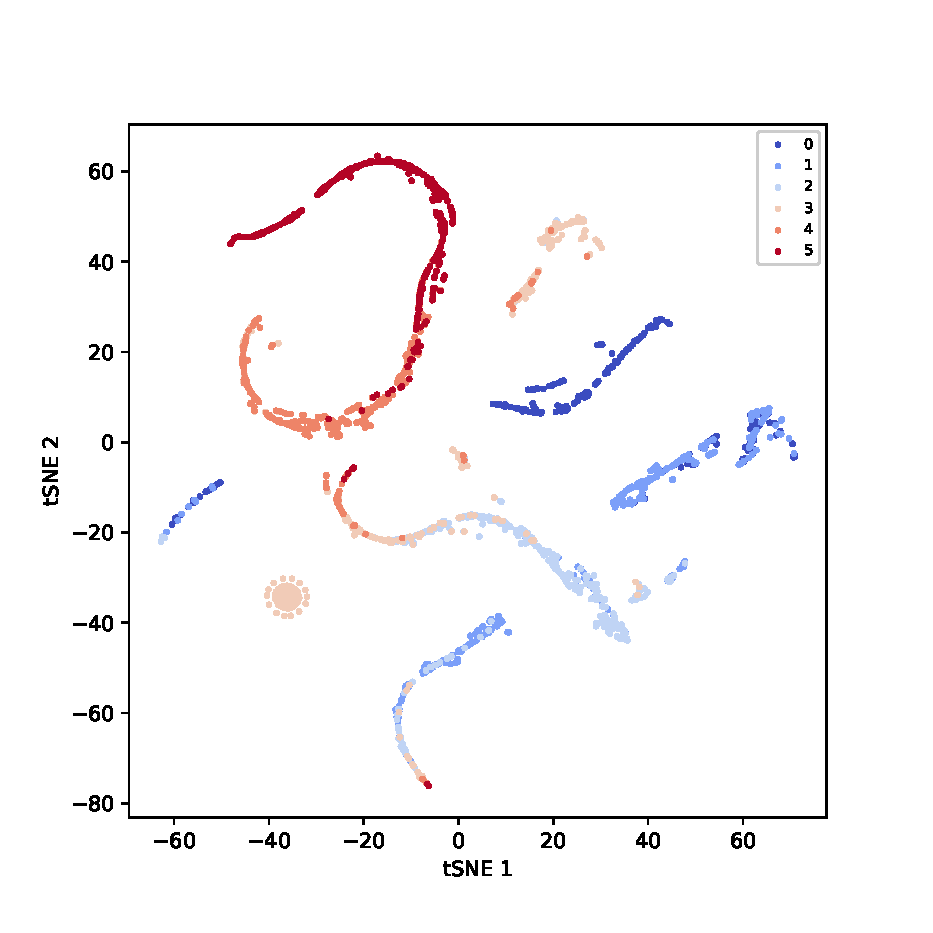
\includegraphics[width=0.36\linewidth]{fig/Cora_1to3_tSNE.eps}
    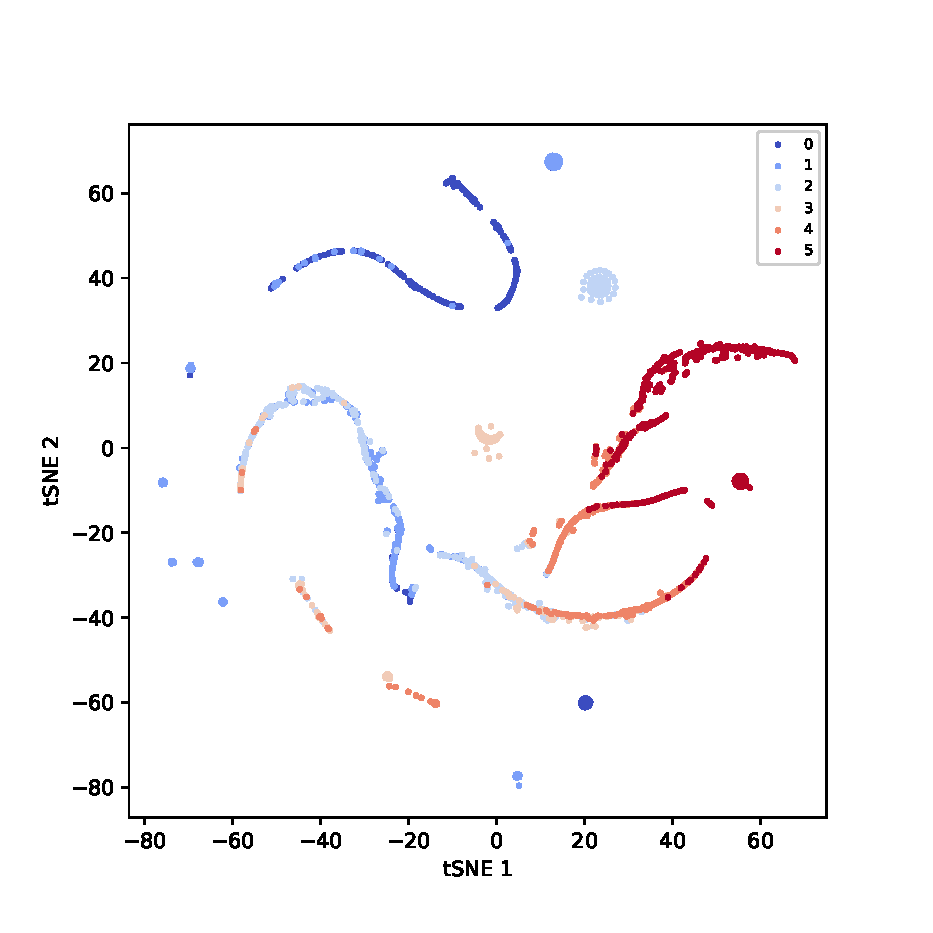
\includegraphics[width=0.36\linewidth]{fig/Citeseer_1to3_tSNE.eps}
    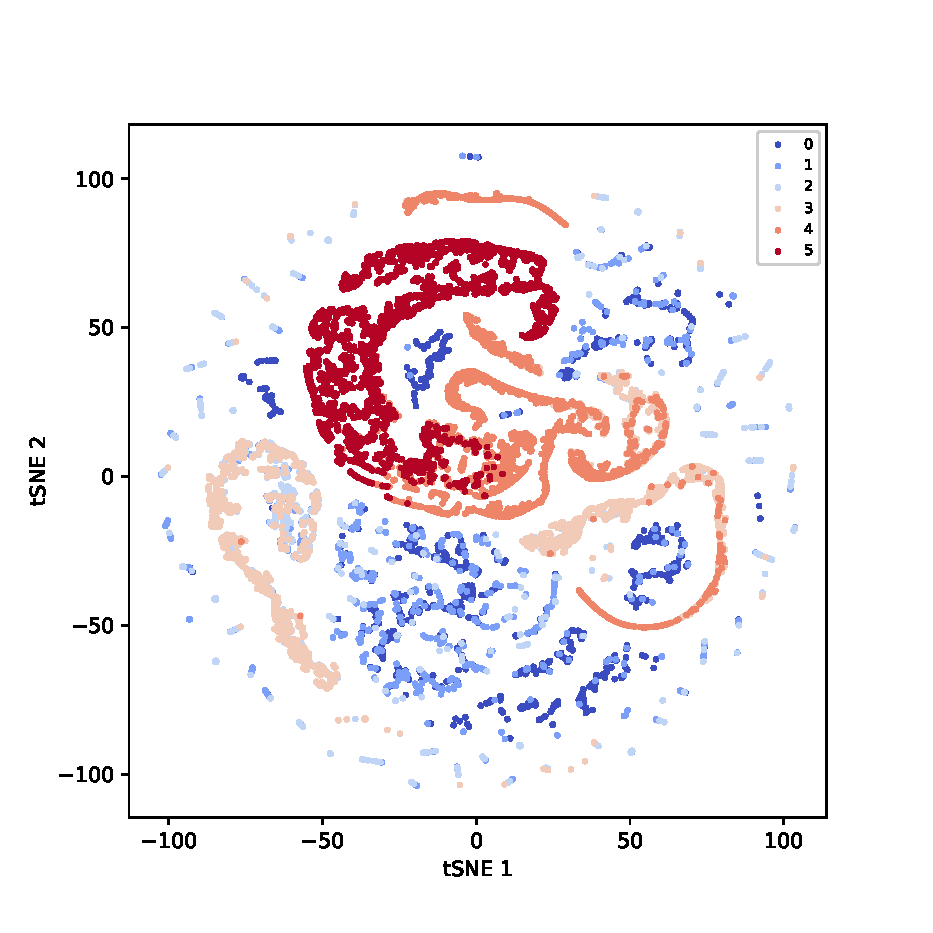
\includegraphics[width=0.36\linewidth]{fig/PubMed_1to3_tSNE.eps}
    \hspace*{-1in}

    \caption{tSNE on graph embeddings with Degree predicting PageRank}
  \hspace*{-1.5in}
    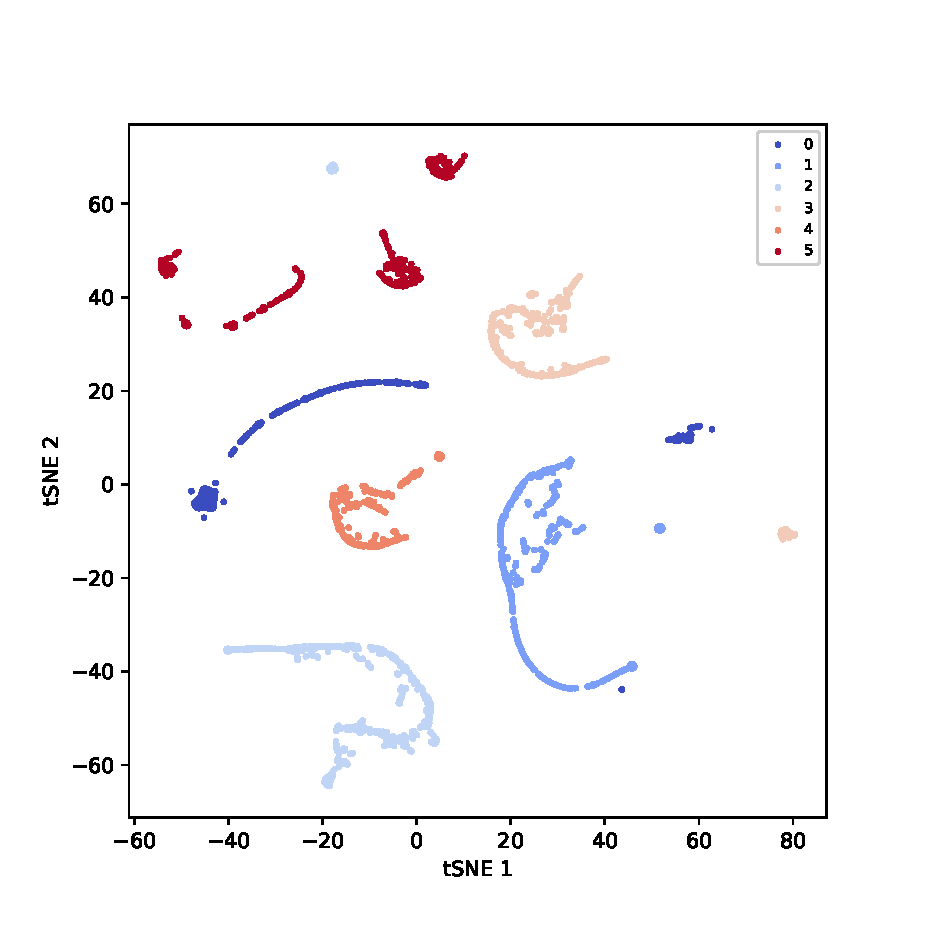
\includegraphics[width=0.35\linewidth]{fig/Cora_2to1_tSNE.eps}
    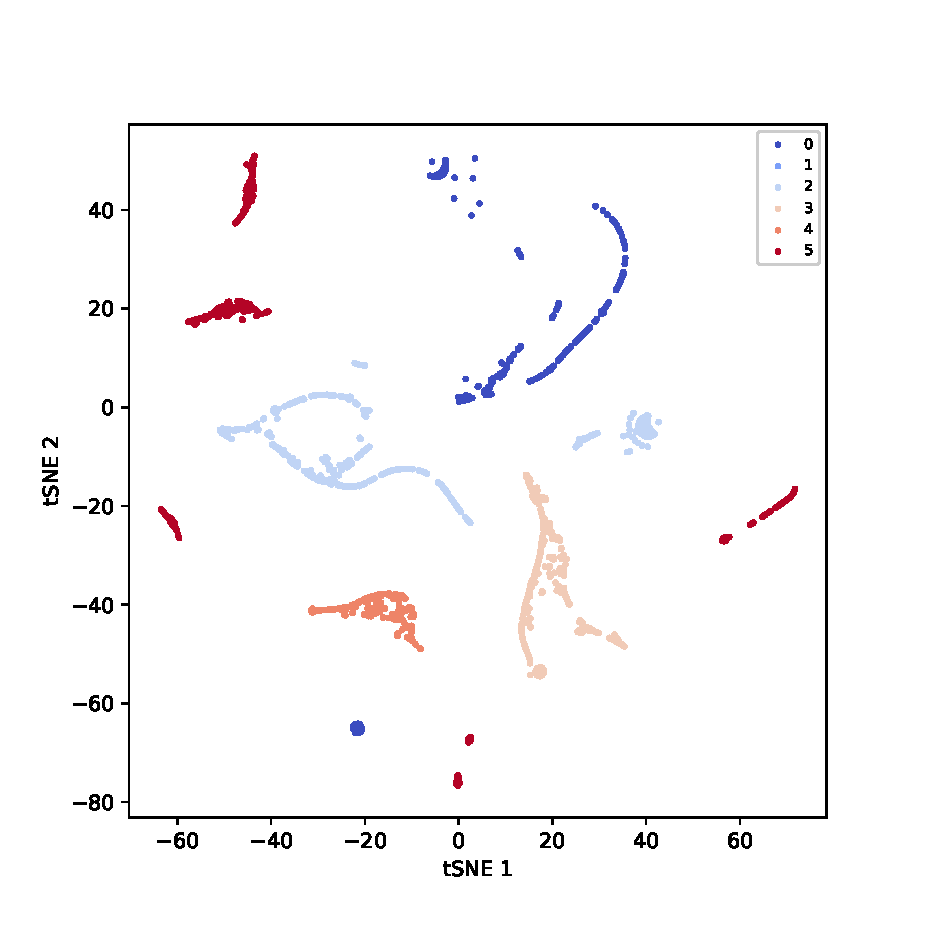
\includegraphics[width=0.35\linewidth]{fig/Citeseer_2to1_tSNE.eps}
    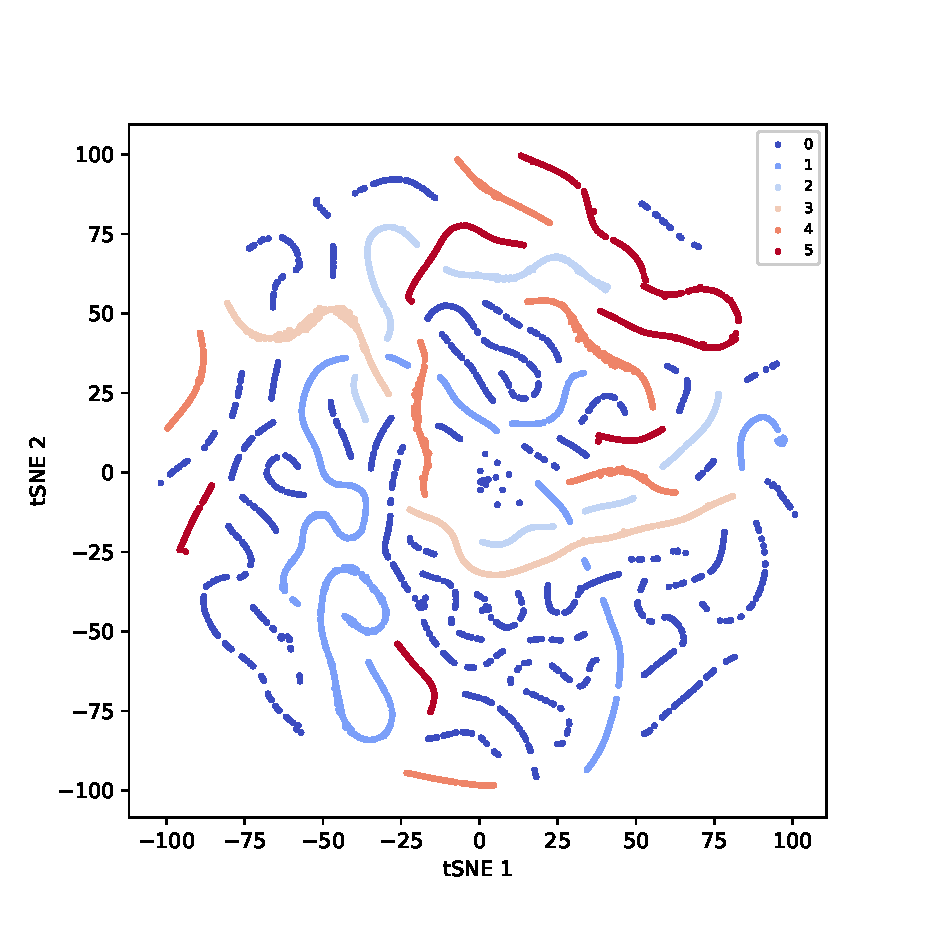
\includegraphics[width=0.35\linewidth]{fig/PubMed_2to1_tSNE.eps}
    \hspace*{-1.5in}

    \caption{tSNE on graph embeddings with Clustering predicting Degree}
\end{center}
\end{figure}







\begin{table*}[htb]
  \caption{Feature to Feature Prediction Results on TUDatasets (bins = 6)}
  \label{tab:commands}
  \begin{tabular}{*{13}{c}} \toprule
{Aim}  & \multicolumn{4}{c}{{\sc NC1}} & \multicolumn{4}{c}{{\sc Proteins}} & \multicolumn{4}{c}{{\sc Enzymes}}\\
\cmidrule(lr){2-5}\cmidrule(lr){6-9}\cmidrule(lr){10-13}
& GCN & GIN & SAGE & GAT & GCN & GIN & SAGE & GAT & GCN & GIN & SAGE & GAT \\ \hline
{1 -> 2} & & & &\\
{1 -> 3} \\
{1 -> 4} \\
{1 -> 5}\\
{2 -> 3}\\
{2 -> 4}\\
{2 -> 5}\\
{3 -> 2} \\	
{4 -> 2} \\
{4 -> 3} \\
{4 -> 5} \\
{5 -> 2} \\
{5 -> 3} \\
{5 -> 4} \\
\bottomrule
  \end{tabular}
\end{table*}


\begin{table}[htb]
  \caption{Hyper-parameter 1 : number of bins}
  \label{tab:commands}
  \begin{tabular}{*{7}{c}} \toprule
{Bins}  & \multicolumn{3}{c}{{\sc Citeseer}} & \multicolumn{3}{c}{{\sc PubMed}} \\
\cmidrule(lr){2-4}\cmidrule(lr){5-7}
& 3->2 & 4->5 & 5->3 & 3->2 & 4->5 & 5->3 \\ \hline
2 & 1.0000& 0.7620& 0.8350 &   \\
3 & 1.0000& 0.6800& 0.7820 &   \\
4 & 1.0000& 0.5640 & 0.7440   \\
5 & 0.9960& 0.5310 & 0.7200   \\
6 & 1.0000& 0.4680 & 0.7250   \\
7 & 1.0000& 0.3870 & 0.7110   \\
8 & 1.0000& 0.3620 & 0.7020   \\
9 & 1.0000& 0.3800 & 0.6910   \\
10 & 1.0000& 0.3910 & 0.6900  \\
\bottomrule
  \end{tabular}
\end{table}




\subsection{Feature Augmentation Results}

\subsection{Additional Features}



\subsection{self-generated graphs}

\paragraph{}

\subsection{Regression tasks}






single \\(finish)
concatenated\\(on-going)
original with concatenated\\(on-going)
GNN and our own model\\(on-going)






Multi-graph input(Graph Classification), we need to compute each graph's property. Batch size is 1 in this case. (Graph classification problem instead of node classification problem)


We have the 


violin plot here and also the rectified-bin algo.

intro  + selected property\\
feature distribution pics\\
comparison by graph \\
set by binning method -> 1)classification or regression 2) how many classes  by binning 3) using normalization or not



innovation1: different from 



\subsection{Comparison between datasets}
visualization, graph and node, and also which is easy to interpret through feature and which not





\section{Conclusions and Discussions}




\paragraph{Future works}







%%
%% The next two lines define the bibliography style to be used, and
%% the bibliography file.
\bibliographystyle{ACM-Reference-Format}
\bibliography{references}

%%
%% If your work has an appendix, this is the place to put it.
\appendix

\end{document}
\endinput
%%
%% End of file `sample-sigconf.tex'.
